%!TEX encoding = UTF-8 Unicode
%!TEX root = ../lect-w08.tex

%%%

\ifkompendium\else

\Subsection{Kontrollskrivning}


% \begin{Slide}{Kontrollskrivning 2019: Vanliga saker som många behöver träna på}
% \begin{itemize}
%   \item iterera över sekvenser med \code{map} och \code{for yield}-uttryck
%   \item om index behövs: använda \code{indices} istället för andra mer felbenägna sätt
%   \item undvika hårdkodning: använd givna konstanter t.ex. \code{NbrOfPegs} och inte \code{5} 
%   \item använda \code{Option}, \code{Some}, \code{None} vid hantering av saknade värden
%   \item booleska uttryck, t.ex. skriva \code{a && b} direkt i stället för \code{if (a && b) true else false}
%   \item inte skapa förlorade värden -- alltså glömt att ta hand om resultat från uttryck som borde varit med i en tilldelning, returvärde el. likn.
% \end{itemize}  
% \end{Slide}

%%% AAAARGH -- version clash ? or something causing thins in Ubuntu 20.04 
%%%   but not in ubuntu 18.04:
%%%
    % Package pgfplots Warning: running in backwards compatibility mode (unsuitable t
    % ick labels; missing features). Consider writing \pgfplotsset{compat=1.16} into 
    % your preamble.
    % on input line 9.

    % No file lect-w08.nav.
    % [1{/var/lib/texmf/fonts/map/pdftex/updmap/pdftex.map}]
    % No file lect-w08.toc.
    % [2] (./body/lect-w08-reboot-camp.tex [3] (./lect-w08.vrb

    % ! Package pgfplots Error: Sorry, could not retrieve column 'poäng' from table 
    % '<inline_table>'. Please check spelling (or introduce name aliases)..

    % See the pgfplots package documentation for explanation.
    % Type  H <return>  for immediate help.
    % ...                                              
                                                      
    % l.26 ...e[x=poäng,y=kamraträttat]{\dataSjutton};
                                                      
    % !  ==> Fatal error occurred, no output PDF file produced!
    % Transcript written on lect-w08.log.


% \begin{Slide}{Resultat på kontrollskrivning 2020}
%   \pgfplotstableread[row sep=\\,col sep=&]{
%       poäng & kamraträttat  \\
%       0     & 4             \\
%       1     & 19            \\
%       2     & 34            \\
%       3     & 21            \\
%       4     & 32            \\
%       5     & 6             \\
%       }\dataSjutton
  
%   \begin{minipage}{0.6\textwidth}
%   \hspace*{-0.65cm}\begin{tikzpicture}[scale=0.9, every node/.style={scale=0.9}]
%       \begin{axis}[
%               ybar,
%               bar width=15,
%               symbolic x coords={0,1,2,3,4,5},
%               xtick=data,
%               nodes near coords,
%               nodes near coords align={vertical},
%               legend style={at={(0.5,1)},anchor=south,legend columns=-1,draw=none},
%               ymin=0,ymax=50,
%               ylabel={Antal},
%               xlabel={Poäng/10},
%           ]
%           \addplot table[x=poäng,y=kamraträttat]{\dataSjutton};
%           \legend{poäng efter korrigering}
%       \end{axis}
%   \end{tikzpicture}
%   \end{minipage}%
%   \begin{minipage}{0.35\textwidth}
%   \begin{itemize}\SlideFontTiny
%   \item[] Totalt: 116 st (100\%) fördelning efter korrigering:
%   \item[] 4 -- 5: 38st (33\%)
%   \item[] 3 -- 5: 59st (51\%)
%   \item[] 0 -- 2: 57st (49\%)
%   \item[] 0 -- 1: 23st (20\%)
%   \item[]
%   \item[] Invändningar: 17 st varav 12 st ändrades
%   \item[] Inga invändningar: 99 st varav 2 st ändrades
  
%   \end{itemize}
%   \end{minipage}%
% \end{Slide}


% \begin{Slide}{Resultat på kontrollskrivning 2019}
%   \pgfplotstableread[row sep=\\,col sep=&]{
%       poäng & kamraträttat  \\
%       0     & 4             \\
%       1     & 28            \\
%       2     & 45            \\
%       3     & 21            \\
%       4     & 14            \\
%       5     & 6             \\
%       }\dataSjutton
  
%   \begin{minipage}{0.6\textwidth}
%   \hspace*{-0.65cm}\begin{tikzpicture}[scale=0.9, every node/.style={scale=0.9}]
%       \begin{axis}[
%               ybar,
%               bar width=15,
%               symbolic x coords={0,1,2,3,4,5},
%               xtick=data,
%               nodes near coords,
%               nodes near coords align={vertical},
%               legend style={at={(0.5,1)},anchor=south,legend columns=-1,draw=none},
%               ymin=0,ymax=50,
%               ylabel={Antal},
%               xlabel={Poäng/10},
%           ]
%           \addplot table[x=poäng,y=kamraträttat]{\dataSjutton};
%           \legend{poäng efter korrigering}
%       \end{axis}
%   \end{tikzpicture}
%   \end{minipage}%
%   \begin{minipage}{0.35\textwidth}
%   \begin{itemize}\SlideFontTiny
%   \item[] Totalt: 117 st (100\%) fördelning efter korrigering:
%   \item[] 4 -- 5: 52st (23\%)
%   \item[] 3 -- 5: 72st (46\%)
%   \item[] 0 -- 2: 53st (54\%)
%   \item[] 0 -- 1: 32st (20\%)
%   \item[]
%   \item[] Invändningar: 24 st varav 20 st ändrades
%   \item[] Inga invändningar:  94 st varav 9 st ändrades
  
%   \end{itemize}
%   \end{minipage}%
% \end{Slide}

\begin{Slide}{Omkontrollskrivning}
  \begin{itemize}
    % \item \Alert{EXTRAUNDERVISNING} för de som har det \Alert{allra svårast}
    % \begin{itemize}
    %   \item Nu på \Emph{torsdag} den 7/11 kl \Alert{8-10} i \Emph{E:2116}
    %   \item Behovsstyrd behandling av grundläggande koncept från lp1.
    %   \item Anmälan: {\small \url{https://forms.gle/996tQWZ8kKeAMFuL7}}
    %   \item De med \textbf{mindre än 15p} på kontrollskrivningen har \Emph{förtur} och rekommenderas \Alert{starkt} att delta!
    %   \item Medtag papper, penna och snabbref.
    % \end{itemize}
    \item \Alert{OMKONTROLLSKRIVNING}\\för de som ej fullföljde ordinarie skrivning:
    \begin{itemize}
      \item Datum meddelas senare. %Måndagen den 16/11 kl 12:15 till ca 16 i Canvas
      %\item Förbered: legitimation, penna, papper, förtäring. %mobil för scanning,. 
      \item Håll koll på mejl och anslag i Canvas.
      %\item Karta till ''glasburen'':{\url{https://fileadmin.cs.lth.se/cs/Bilder/Salar/E2405.pdf} }
    \end{itemize}
  \end{itemize}
\end{Slide}

% \begin{Slide}{Resultat på kontrollskrivning 2019}
%     \pgfplotstableread[row sep=\\,col sep=&]{
%         poäng & kamraträttat & korrigerat\\
%         0     & 4            & 2  \\
%         1     & 28           & 22 \\
%         2     & 45           & 40 \\
%         3     & 21           & 27 \\
%         4     & 14           & 18 \\
%         5     & 6            & 9  \\
%         }\dataSjutton
    
%     \begin{minipage}{0.6\textwidth}
%     \hspace*{-0.65cm}\begin{tikzpicture}[scale=0.9, every node/.style={scale=0.9}]
%         \begin{axis}[
%                 ybar,
%                 symbolic x coords={0,1,2,3,4,5},
%                 xtick=data,
%                 nodes near coords,
%                 nodes near coords align={vertical},
%                 legend style={at={(0.5,1)},anchor=south,legend columns=-1,draw=none},
%                 ymin=0,ymax=50,
%                 ylabel={Antal},
%                 xlabel={Poäng/10},
%             ]
%             \addplot table[x=poäng,y=kamraträttat]{\dataSjutton};
%             \addplot table[x=poäng,y=korrigerat]{\dataSjutton};
%             \legend{kamraträttat, korrigerat}
%         \end{axis}
%     \end{tikzpicture}
%     \end{minipage}%
%     \begin{minipage}{0.35\textwidth}
%     \begin{itemize}\SlideFontTiny
%     \item[] Totalt: 117 st (100\%) fördelning efter korrigering:
%     \item[] 4 -- 5: 52st (23\%)
%     \item[] 3 -- 5: 72st (46\%)
%     \item[] 0 -- 2: 53st (54\%)
%     \item[] 0 -- 1: 32st (20\%)
%     \item[]
%     \item[] Invändningar: 24 st varav 20 st ändrades
%     \item[] Inga invändningar:  94 st varav 9 st ändrades
    
%     \end{itemize}
%     \end{minipage}%
% \end{Slide}
    
    

% \begin{Slide}{Resultat på kontrollskrivning 2018}
% \pgfplotstableread[row sep=\\,col sep=&]{
%     poäng & kamraträttat & korrigerat\\
%     0     & 5            & 5\\
%     1     & 31           & 27 \\
%     2     & 18           & 21\\
%     3     & 27           & 20 \\
%     4     & 34           & 37 \\
%     5     & 10           & 15 \\
%     }\dataSjutton

% \begin{minipage}{0.6\textwidth}
% \hspace*{-0.65cm}\begin{tikzpicture}[scale=0.9, every node/.style={scale=0.9}]
%     \begin{axis}[
%             ybar,
%             symbolic x coords={0,1,2,3,4,5},
%             xtick=data,
%             nodes near coords,
%             nodes near coords align={vertical},
%             legend style={at={(0.5,1)},anchor=south,legend columns=-1,draw=none},
%             ymin=0,ymax=50,
%             ylabel={Antal},
%             xlabel={Poäng/10},
%         ]
%         \addplot table[x=poäng,y=kamraträttat]{\dataSjutton};
%         \addplot table[x=poäng,y=korrigerat]{\dataSjutton};
%         \legend{kamraträttat, korrigerat}
%     \end{axis}
% \end{tikzpicture}
% \end{minipage}%
% \begin{minipage}{0.35\textwidth}
% \begin{itemize}\SlideFontTiny
% \item[] Totalt: 125 st (100\%) fördelning efter korrigering:
% \item[] 4 -- 5: 52st (42\%)
% \item[] 3 -- 5: 72st (58\%)
% \item[] 0 -- 2: 53st (42\%)
% \item[] 0 -- 1: 32st (26\%)
% \item[]
% \item[] Invändningar: 30 st varav 16 st ändrades
% \item[] Inga invändningar:  95 st varav 4 st ändrades

% \end{itemize}
% \end{minipage}%
% \end{Slide}





% \begin{Slide}{Resultat på kontrollskrivning 2017}
% \pgfplotstableread[row sep=\\,col sep=&]{
%     poäng & kamraträttat & korrigerat\\
%     0     & 10  & 4\\
%     1     & 28  & 31 \\
%     2     & 20  & 19\\
%     3     & 22  & 21 \\
%     4     & 17  & 18 \\
%     5     & 17  & 22 \\
%     }\dataSjutton

% \begin{minipage}{0.6\textwidth}
% \hspace*{-0.65cm}\begin{tikzpicture}[scale=0.9, every node/.style={scale=0.9}]
%     \begin{axis}[
%             ybar,
%             symbolic x coords={0,1,2,3,4,5},
%             xtick=data,
%             nodes near coords,
%             nodes near coords align={vertical},
%             legend style={at={(0.5,1)},anchor=south,legend columns=-1,draw=none},
%             ymin=0,ymax=50,
%             ylabel={Antal},
%             xlabel={Poäng/10},
%         ]
%         \addplot table[x=poäng,y=kamraträttat]{\dataSjutton};
%         \addplot table[x=poäng,y=korrigerat]{\dataSjutton};
%         \legend{kamraträttat, korrigerat}
%     \end{axis}
% \end{tikzpicture}
% \end{minipage}%
% \begin{minipage}{0.35\textwidth}
% \begin{itemize}\SlideFontTiny
% \item[] Totalt: 115 st (100\%) fördelning efter korrigering:
% \item[] 4 -- 5: 40st (34\%)
% \item[] 3 -- 5: 61st (53\%)
% \item[] 0 -- 2: 54st (47\%)
% \item[] 0 -- 1: 35st (30\%)
% \end{itemize}
% \end{minipage}%
% \end{Slide}



% \begin{Slide}{Resultat på kontrollskrivning 2016}
% \pgfplotstableread[row sep=\\,col sep=&]{
%     poäng & kamraträttat & korrigerat\\
%     0     & 18  & 15\\
%     1     & 29  & 29 \\
%     2     & 17  & 15\\
%     3     & 20  & 21 \\
%     4     & 21  & 18 \\
%     5     & 8   & 15 \\
%     }\dataSexton

% \begin{minipage}{0.6\textwidth}
% \hspace*{-0.65cm}\begin{tikzpicture}[scale=0.9, every node/.style={scale=0.9}]
%     \begin{axis}[
%             ybar,
%             symbolic x coords={0,1,2,3,4,5},
%             xtick=data,
%             nodes near coords,
%             nodes near coords align={vertical},
%             legend style={at={(0.5,1)},anchor=south,legend columns=-1,draw=none},
%             ymin=0,ymax=50,
%             ylabel={Antal},
%             xlabel={Poäng/10},
%         ]
%         \addplot table[x=poäng,y=kamraträttat]{\dataSexton};
%         \addplot table[x=poäng,y=korrigerat]{\dataSexton};
%         \legend{kamraträttat, korrigerat}
%     \end{axis}
% \end{tikzpicture}
% \end{minipage}%
% \begin{minipage}{0.35\textwidth}
% \begin{itemize}\SlideFontTiny
% \item[] Totalt: 107 st (100\%) fördelning efter korrigering:
% \item[] 4 -- 5: 33st (29\%)
% \item[] 3 -- 5: 54st (48\%)
% \item[] 0 -- 2: 59st (52\%)
% \item[] 0 -- 1: 44st (39\%)
% \end{itemize}
% \end{minipage}%
% \end{Slide}




\Subsection{REBOOT CAMP}

\begin{Slide}{Reboot Camp}

\begin{itemize}
  \item
  Träffas i din samarbetsgrupp och organisera själva en \Emph{REBOOT CAMP} baserat på kontrollskrivningsresultatet.

  \begin{itemize}
    \item Hur gick kontrollskrivningen?
    \item Hur använde du tiden?
    \item Hur påverkar det du nu vet om bedömningen hur kunde använt tiden bättre?
  \end{itemize}
  
  % \item \Alert{EXTRAUNDERVISNING} för de som har det \Alert{allra svårast}
  % \begin{itemize}
    %   \item Nu på \Emph{torsdag} den 7/11 kl \Alert{8-10} i \Emph{E:2116}
    %   \item Behovsstyrd behandling av grundläggande koncept från lp1.
    %   \item Anmälan: {\small \url{https://forms.gle/996tQWZ8kKeAMFuL7}}
    %   \item De med \textbf{mindre än 15p} på kontrollskrivningen har \Emph{förtur} och rekommenderas \Alert{starkt} att delta!
    %   \item Medtag papper, penna och snabbref.
    % \end{itemize}
    
    \item \Emph{Diskutera med handledare} hur du din studieteknik ev. kan förbättras med ledning av kontrollskrivningsresultatet.
    %\item \Emph{STAY CALM} 
    %\item \Alert{GET ON TRACK}
\end{itemize}


\end{Slide}

%
% \begin{Slide}{Omplanering: w08 = REBOOT CAMP}\SlideFontSmall
% Det är \Alert{för många} som ligger \Alert{för långt efter}: \\
% \Emph{Vi måste göra något!}
% \begin{itemize}
% \item Omplanering: w08 = REBOOT CAMP
% \begin{itemize}\SlideFontTiny
% \item \Alert{GE JÄRNET} för att stärka dig inför resten av kursen!
% \item Noggrann genomgång av kontrollskrivning
% \item Gör självdiagnostik och kämpa dig över trösklar och fyll igen luckor
% \item Slipa dina inlärningsverktyg!
% \item Resurstider: \code{reboot-init}: \Emph{planera, arbeta}
% \item Labb: \code{reboot-check}: \Emph{visa hur det går, arbeta}
% \end{itemize}
% \item Vi senarelägger alla kvarvarande labbar en vecka så att w08 frigörs;
%  lab \code{chords-team} görs alltså i vecka w09 etc.
%
% \item Sista labben \code{life} omdefinieras till att ingå bland projektalternativen i slutet av kursen (man får ändå öva på matriser på lab \code{maze})
%
% \item Stoffet i veckorna w12 \& w13 slås ihop och minskas ned
%
% \item Övn threads blir frivilligt extramaterial och ingår ej i examinationen.
%
% \end{itemize}
% \end{Slide}


%\Subsection{Slipa verktygen}



% \begin{Slide}{Slipa verktygen}
% För dig som har det \Alert{svårt}:
% \begin{itemize}
% \item Man kan inte lära sig ett språk bara genom att \Alert{passivt} läsa
% \item Om du inte börjat än: nu måste du verkligen börja skriva, prata, uppfinna, konstruera, göra själv, vara \Emph{aktiv}, ...
% \end{itemize}
% För dig som har det \Emph{lätt}:
% \begin{itemize}
% \item Om du utmanar dig når du \Emph{mycket} längre
% \item Analysera dina styrkor och svagheter
% \item Utveckla din studieteknik och problemlösningsförmåga
% \end{itemize}
% \end{Slide}
%
% \begin{Slide}{Vad avgör studieframgång?}
% Studieteknik, Attityd till sina studier, (Talang)
% \url{https://www.youtube.com/watch?v=gSbpRjxYq24}
%
% \vspace{2em} Att repetera:
% \url{https://www.youtube.com/watch?v=mmAmsaRH_VA}
%
% \vspace{2em} Att planera:
% \url{https://www.youtube.com/watch?v=g2BTFzYnNNY}
% \end{Slide}

\begin{Slide}{Självdiagnostik och planering}
\begin{itemize}
  \item Vad behöver jag extra träning på?
  \begin{itemize}
    \item Vad hade jag lätt resp. svårt för på kontrollskrivingen?
    \item Vilka är mina \Alert{trösklar}? Extra svårt?
    \item Vilka är mina \Alert{luckor}? Inte provat alls?
    \item Vilka är mina \Emph{intressen}? Hur fördjupa mig?
  \end{itemize}
  \item Hur ska jag plugga?
  \begin{itemize}
    \item Gör ett schema dag för dag.
    \item Dela upp varje pass i delar: teori, övningar, labbar. 
    \item Övningarnas syfte: att utöka din verktygslåda.
    \item Identifiera övningar från lp1 om det du behöver träna på.
    \item Du som fick 0-2: gå på minst 1 extra online-resurstider per vecka.
  \end{itemize}
\end{itemize}
\end{Slide}

{\setbeamercolor{background canvas}{bg=black}
\frame[plain]{\centering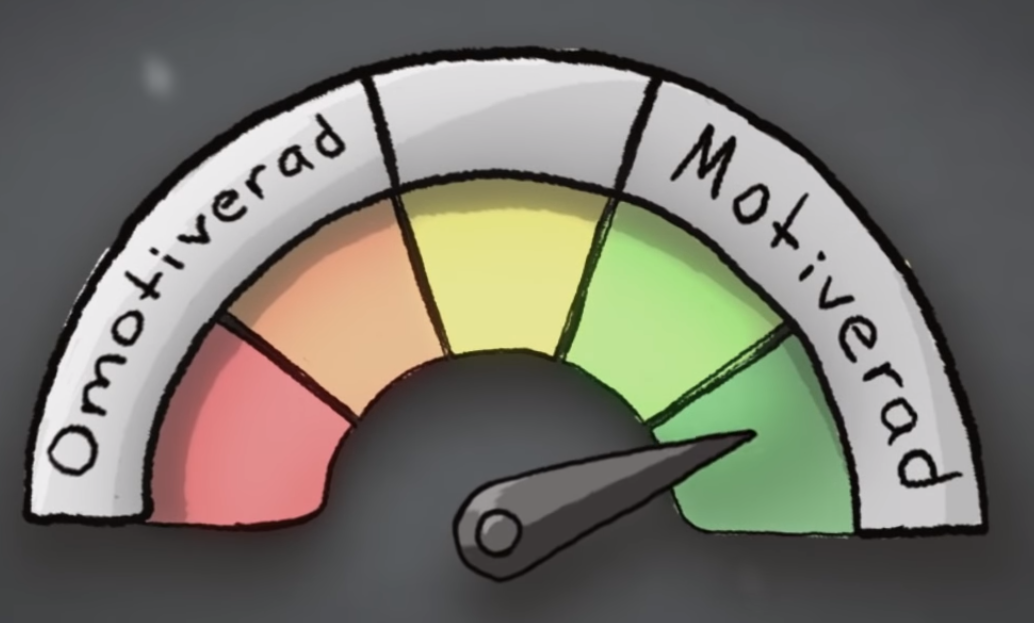
\includegraphics[width=1.0\textwidth]{../img/motivation.png}}
}

% \begin{Slide}{Strategier för problemlösning i programmering}
% \begin{itemize}
% \item Börja med ett litet men fungerande program; ta sedan många små steg och testa hela tiden att det fungerar
% \item Om problemet är för \Alert{svårt}:\\ lös först ett \Emph{lättare}, relaterat problem
% \item Dela upp problemet i delar
% \begin{itemize}
% \item \code{val braNamn = delresultat}
% \item \code{def delLösning = algoritm som löser delproblem}
% \item \code{??? // inte klart än}
% \end{itemize}
% \item Problemlösning är inte linjärt: du måste kunna knåpa på ditt program i olika ''ändar''; skriva lite här och där; stoppa in; flytta runt; ändra
% \end{itemize}
% \end{Slide}
%
% \begin{Slide}{Strategier för att komma över trösklar}\SlideFontSmall
% \Alert{tröskel} == jag har svårt att begripa och komma vidare; kan ej själv konstruera
%
% \begin{itemize}\SlideFontTiny
% \item Du måste först \Emph{identifiera tröskeln} och tydligt formulera vad du inte förstår eller inte kan klara av att själv skapa.
%
% \item Du måste hitta ett sätt att \Emph{konkretisera} begrepp och \Emph{visualisera} vad som händer \\
% Använd analogier: kaffekvarnen för funktion, stämpla för instansiering, etc.
%
% \item Använd flera exempel på samma sak: försök se \Emph{mönster} \\
% Exempel: Tomat och Gurka är Grönsak; Student och Lärare är Person. \\ Lär dig pseudokodexempel på vanliga algoritmer i kompendiet utantill!
%
% \item Gör \Emph{enklast möjliga} exempel som du exekverar: \\ Skapa en enkel klass med bara en heltalsmedlem och ''lek'' med den.
%
% \item Bygg vidare på det du lär dig och \Emph{utvidga} stegvis med större exempel.\\ Exekvera allt större kod som du själv skriver!
%
% \item \Emph{Avancera}: Kombinera med begrepp du redan känner. Exekvera!
%
% \end{itemize}
% Utgå från det du vet om hur just \Emph{du} lär dig bäst. Hur ska du vara \Alert{aktiv}? \\ Rita. Prata. Skriv sammanfattningar. Skapa egna program. ...
% \end{Slide}
%
% \begin{Slide}{Uppdrag under rasten}
% \begin{itemize}
% \item Tala med med en eller två som är \Emph{ungefär på din nivå} med ledning av resultatet på kontrollskrivningen. (Eller skriv ner för dig själv om du helst vill vara ensam)
%
% \item 5 minuter var: berätta för den andre om...
% \begin{itemize}
%  \item dina trösklar: vad är extra svårt?
%  \item dina luckor: vad har jag inte ens provat själv?
%  \item dina fördjupningsintressen: vad vill jag veta mer om?
%  \item övningar och laborationer som behöver kompletteras
% \end{itemize}
% \item \Alert{Fastna inte} i orsaker/ursäkter till situationen: \Emph{utgå från nuläget} och  indentifiera trösklar/luckor/fördjupning
% \end{itemize}
% \end{Slide}
%
%
% \begin{Slide}{Tillbaka efter rasten:}
% %Påbörja detta arbete som du sedan fortsätter med i eftermiddag/kväll:
% \begin{itemize}
% \item Gör en lista på vad just \Alert{du} behöver göra för att \Emph{slipa dina verktyg} i programmering?
% \item För varje begreppslista i w01-w07:
% \begin{itemize}
% \item Välj ut några begrepp som är viktiga för dig att träna mer på.
% \item Välj ut några övningar som är kopplade till begreppen.
% \item Gör en \Emph{prio-lista} för begreppen/övningarna.
% \item Planera ditt arbete för veckan:
% \begin{itemize}
% \item Övningar
% \item Ev. labbar att komplettera
% \end{itemize}
% \end{itemize}
% \item Ta med dig \Emph{prio-listan} till \Alert{resurstiderna} och diskutera med handledare!
% \end{itemize}
% \end{Slide}
%
%
% %\Subsection{Prioritera dina uppgifter}
%
% \begin{Slide}{Inventering av trösklar, luckor, fördjupning}
% I ditt arbete med att identifiera trösklar, luckor, fördjupning kan du använda:
% \begin{itemize}
% \item Kontrollskrivningen
% \item Målen på övningarna
% \item Begreppslistan i varje modul
% \end{itemize}
% Gör en inventering och markera det du har någorlunda koll på och det du tycker är extra svårt (tröskel) eller sådant du missat (luckor). Om du är redo för fördjupning markera intressanta delar att lära dig mer om.
% \end{Slide}
%
% \begin{Slide}{Prioritera och definiera dina anpassade träning}
% \begin{itemize}
% \item Gör klart eventuella labbar som behöver kompletteras.
% \item Välj en lagom stor mängd övningar ur kompendiet som hjälper dig med trösklar och luckor. Modifiera gärna övningarna efter dina behov.
% \item Definiera ett program du ska jobba med fram till och med reboot-check.
% \end{itemize}
% \end{Slide}

% \begin{Slide}{Hur blir jag godkänd på reboot-check?}
% \begin{itemize}
% \item Förbered en kort genomgång som du ska göra när du får tid med handledare:
% \begin{itemize}
% \item Vilka trösklar/luckor/fördjupningar har du identifierat?
% \item Vad har du gjort under veckan?
% \item Visa ditt program som du jobbar med under labben och förklara hur programmet hänger ihop med dina trösklar/luckor/fördjupningar?
% \end{itemize}
% \item Använd tiden under labben till något vettigt;  jobba vidare på ditt eget program medan du väntar.
% \end{itemize}
% Du blir godkänd om du kan resonera om kopplingen mellan dina behov och dina åtgärder.
% \end{Slide}

\fi
